\documentclass[fleqn]{beamer}

\usepackage{algorithm}
\usepackage{algorithmic}
\usepackage{appendixnumberbeamer}
\usepackage{color, colortbl}
\usepackage{amstext}
\usepackage{relsize}

\usepackage{amsmath,amssymb}
\usepackage{epsf}
\usepackage{graphicx}
\usepackage{tabularx}
\usepackage{hyperref}
\usepackage{movie15}
% \usepackage{media9}                                                           
\usepackage[fleqn]{nccmath}
\usepackage{color, colortbl}

\usepackage[encapsulated]{CJK}
\usepackage{ucs}
\usepackage[utf8x]{inputenc}

\usefonttheme[onlylarge]{structurebold}
\setbeamerfont*{frametitle}{size=\normalsize,series=\bfseries}
\setbeamertemplate{navigation symbols}{}

\renewcommand\arraystretch{1.5}

% use one of bsmi(trad Chinese), gbsn(simp Chinese), min(Japanese), mj(Korean); see:
% /usr/share/texmf-dist/tex/latex/cjk/texinput/UTF8/*.fd

\newcommand{\cntext}[1]{\begin{CJK}{UTF8}{gbsn}#1\end{CJK}}
\newcommand{\textkai}[1]{\begin{CJK}{UTF8}{gkai}#1\end{CJK}}
\definecolor{shadow}{gray}{0.8}
\newcommand{\redc}[1]{{\color{red} #1}}
\newcommand{\bluec}[1]{{\color{blue} #1}}
\newcommand{\shadowc}[1]{{\color{shadow} #1}}
\newcommand{\blackc}[1]{{\color{black} #1}}
\newcommand{\whitec}[1]{{\color{white} #1}}
\definecolor{myyellow}{HTML}{FFB700}
\newcommand{\yellowc}[1]{{\color{myyellow} #1}}
\newcommand{\greenc}[1]{{\color{green} #1}}
\newcommand{\vect}[1]{\textbf{\textit{#1}}}
\newcommand{\dd}[0]{\textrm{d}}
\newcommand{\corr}{C^{(3)}}
\newcommand{\fe}{u}

\newcommand{\mh}{\mathcal H}
\newcommand{\slip}{{\textrm{slip}}}
\newcommand{\eps}{\varepsilon}
\newcommand{\ml}{\mathcal L}
\newcommand{\mt}{\mathcal T}
\newcommand{\mo}{\mathcal O}
\newcommand{\mi}{\mathcal I}
\newcommand{\mc}{\mathcal C}
\newcommand{\pathmeas}{\mathcal P}
\newcommand{\proj}{\mathit\Pi}
\newcommand{\fwg}{{\mathcal A}}
\newcommand{\bwg}{{\mathcal B}}
\newcommand{\bsigma}{\boldsymbol\sigma}
\newcommand{\inv}{{\textrm{inv}}}

\usetheme{Warsaw}
% \usetheme{Boadilla}

\begin{document}
\cntext{
  
%% ------------------------------------------  
\title{微观尺度流体力学边界条件的确定}
\author{{{王涵}} }
\institute{中物院高性能数值模拟软件中心~~金属材料团队\\
  \vskip.5cm
\textkai{合作者:陈书宇\ 博士 (HKUST),钱铁铮\  教授 (HKUST),沈平\ 教授 (HKUST) }}
\date{\footnotesize 2015年2月}
\frame{\titlepage}
%%------------------------------------------

%% ------------------------------------------

\begin{frame}{背景介绍}
  \begin{figure}
    \centering
    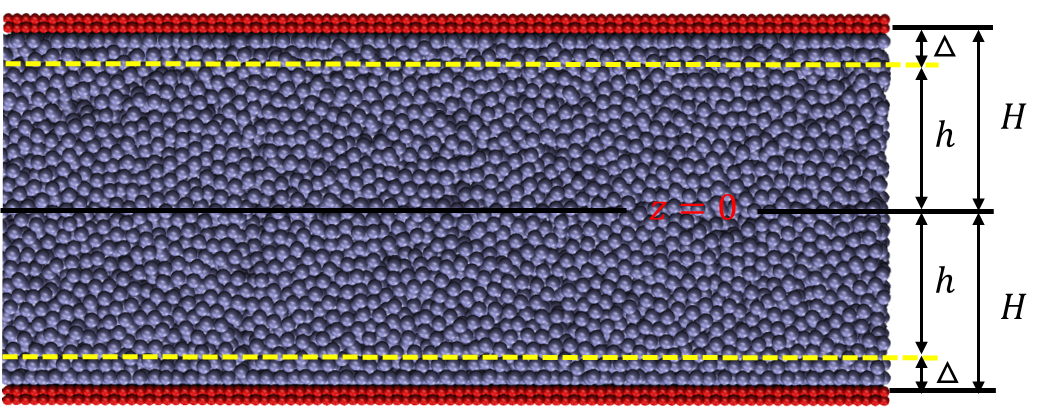
\includegraphics[width=0.9\textwidth]{fig/system.png}
  \end{figure}
  \begin{itemize}
  \item <1-> \bluec{$H$}: 固壁位置。\bluec{$h$}:流体力学区域。\bluec{$\Delta = H - h$}。
  \item <2-> 为简化问题,我们只考虑流体横向流动. 
  \item <3-> 记横向动量密度为 \bluec{$J(z,t) = \rho_0 v(z,t)$}.
  \end{itemize}
\end{frame}

\begin{frame}{宏观边值问题}
  \begin{itemize}
    \vfill
  \item <1-> 求解不可压 Navier-Stokes 方程:
    \begin{align*}
      \bluec{
      \frac{\partial}{\partial t} J(z,t) = \frac{\eta}{\rho_0} \frac{\partial^2}{\partial z^2} J(z,t)
      }
    \end{align*}
    \vfill
  \item <2-> 使用分离变量法,假设 \bluec{ $J(z,t) = Z(z) T(t)$}, 带入 NS 方程,可得
    \begin{align*}
      \bluec{\frac{1}{Z(z)} \frac{d^2 Z(z)}{dz^2} + k^2 = 0} \\
      \bluec{\frac{\rho_0}{\eta T(t)} \frac{d T(t)}{dt} + k^2 = 0}
      % \bluec{\frac{1}{Z_n(z)} \frac{d^2 Z_n(z)}{dz^2} + k_n^2 = 0} \\
      % \bluec{\frac{\rho_0}{\eta T_n(t)} \frac{d T_n(t)}{dt} + k_n^2 = 0}
    \end{align*}
    \vfill
  \end{itemize}
\end{frame}

\begin{frame}{特征值和特征向量}
  \begin{itemize}
    \vfill
  \item <1-> 记第 $n$ 个特征值为 \redc{$k_n$}. 
    \vfill
  \item <2-> 则求解特征问题可得特征向量
    \bluec{
      \begin{align*}
        Z_n(z) &= A_n \sin(k_n z)\\
        T_n(t) &= T_n(0) e^{-\eta k_n^2 t/\rho_0}
      \end{align*}
    }
    \vfill
  \end{itemize}
\end{frame}

\begin{frame}{边界条件}
  \begin{itemize}
  \item <1->
    边界滑移速度 \bluec{$v_n^\slip$} 定义为:
    \bluec{
      \begin{align*}
        \rho_0 v_n^\slip = A_n \sin(k_n h)
      \end{align*}
    }      
  \item <2-> 边界对流体的摩擦应力和流体的粘性应力在边界处平衡:
    \bluec{
      \begin{align*}
        -\beta \rho_0 v_n^\slip = \eta A_n k_n \cos (k_n h)
      \end{align*}
    }
  \item <3->
    \begin{minipage}[t]{0.53\linewidth}
    引入滑移长度 \redc{$l_\slip = \eta / \beta $}, 
    \begin{align*}
      \only<4->{\bluec{\tan (k_n h) = -k_n l_\slip}}
    \end{align*}
    \end{minipage}
    \begin{minipage}[t]{0.43\linewidth}
      \vskip -.8cm
      \begin{figure}
        \centering
        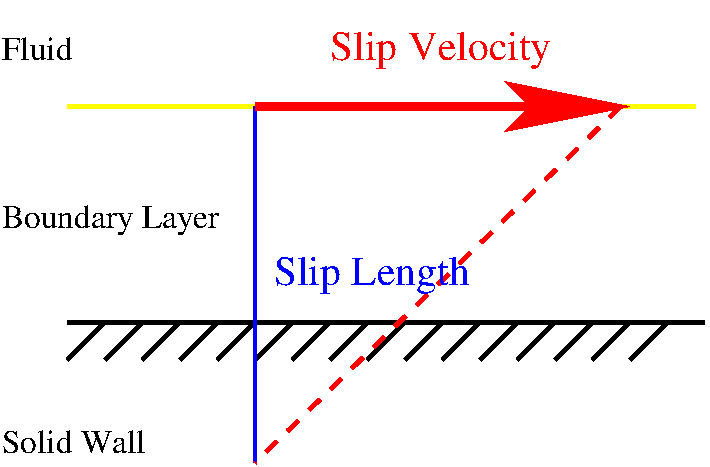
\includegraphics[width=1.0\textwidth]{fig/slip-length.pdf}
      \end{figure}  
    \end{minipage}
  \end{itemize}
\end{frame}

\begin{frame} {求解特征值}
  \begin{itemize}    
  \item <1-> 定义速度场在对偶空间的分量为:
    \bluec{
      \begin{align*}
        \hat v(k, t) = \sum_{i=1}^N v_i(t) \sin(k z_i(t))
      \end{align*}
    }
  \item <2->考察自相关函数:
    \bluec{
      \begin{align*}
        C(k,\Delta t) =
        \frac { \Big\langle \hat v(k,0)\cdot \hat v(k,\Delta t)   \Big\rangle } {\Big\langle \hat v(k,0)\cdot \hat v(k,0)   \Big\rangle }
      \end{align*}
    }  
  \item <3-> 根据线性相应理论:
    \redc{
    \begin{align*}
      C(k_n, \Delta t) = \frac{T_n(\Delta t)}{ T_n(0) }  = e^{-\eta k_n^2 \Delta t / \rho_0}, \quad \tau_n = \rho_0 / k_n^2\eta
    \end{align*}
    }
  \end{itemize}
\end{frame}

% \begin{frame}{自相关函数}
%   \bluec{
%     \begin{align*}
%       &\ln C(k_n, \Delta t) = -\eta k_n^2/\rho_0 \cdot \Delta t,\qquad
%     \end{align*}
%   }
%   \begin{figure}
%     \centering
%     \includegraphics[width=0.7\textwidth]{fig/lnC.png}
%   \end{figure}
% \end{frame}


% \begin{frame} {测试问题描述}
%   \begin{itemize}
%   \item Lennard-Jones 相互作用:
%     \bluec{
%       \begin{align*}
%         U_{ij} = 4\eps_{ij}
%         \Big[
%         \Big(\frac{\sigma_{ij}}{r}\Big)^{12}
%         - \delta_{ij}\Big(\frac{\sigma_{ij}}{r}\Big)^{6}
%         \Big]
%       \end{align*}}
%   \item 模拟参数:
%   \begin{table}
%     \centering
%   \begin{tabular*}{0.8\textwidth}{@{\extracolsep{\fill}}lrr}\hline\hline
%       & 亲水固壁& 厌水固壁 \\\hline
%       $\varepsilon_{ff}$ & $\varepsilon$ & $\varepsilon$ \\
%       $\varepsilon_{wf}$ & $1.16\varepsilon$ & $1.16\varepsilon$ \\
%       $\sigma_{ff}$ & $\sigma$ & $\sigma$\\
%       $\sigma_{wf}$ & $1.04\sigma$ & $1.04\sigma$\\
%       $\delta_{wf}$ & 1.0 & 0.7\\\hline\hline
%     \end{tabular*}
%   \end{table}
%   \end{itemize}
% \end{frame}


\begin{frame}
  \begin{minipage}[t]{0.58\linewidth}
    \vskip -.3cm
    \begin{figure}
      \centering
      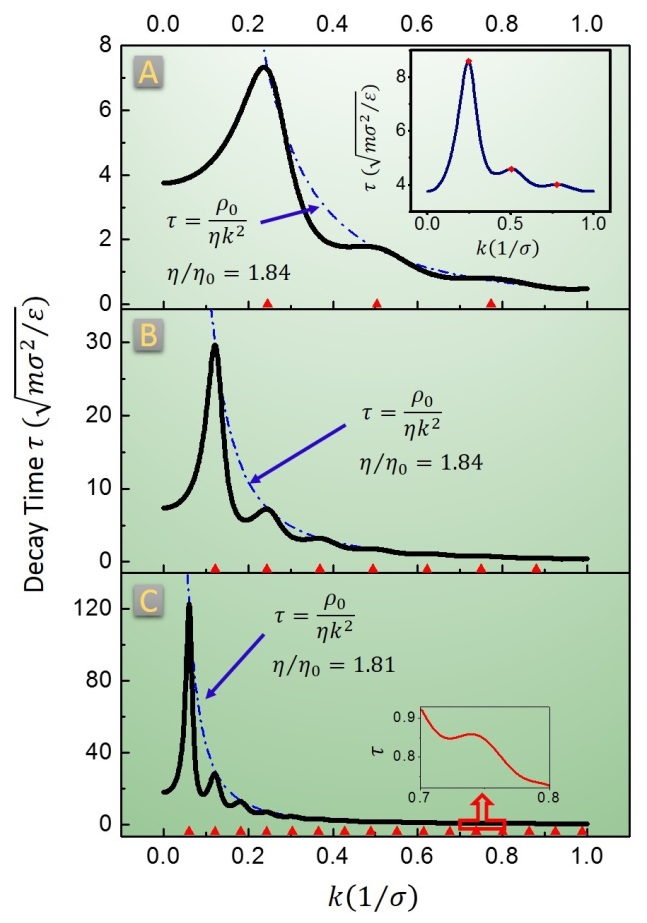
\includegraphics[width=0.99\textwidth]{fig/tau.png}
    \end{figure}      
  \end{minipage}
  \begin{minipage}[t]{0.4\linewidth}
    \begin{itemize}
      \itemsep .2cm
    \item 体系规模:
      \bluec{$H = 13.2\sigma$}\\
      \bluec{$H = 26.1\sigma$}\\
      \bluec{$H = 51.9\sigma$}\\
    \item <2-> 对每个模 \bluec{$k$} 计算衰减时间。
    \item <3-> 确定特征值 \bluec{ $k_n$}.
    \item <4-> 拟合 \bluec{$\eta$}.
    \item <5-> 由特征向量正交性计算 \bluec{$h$}.
    \item <6-> 由特征方程计算滑移长度 \bluec{$l_\slip$}.
    \item <7-> 由$\bluec{\tan (k_n h) = -k_n l_\slip}$反推并验证特征值。
      \end{itemize}
  \end{minipage}
\end{frame}

\begin{frame}{模拟结果} {亲水固壁}
  \begin{figure}
    \centering
    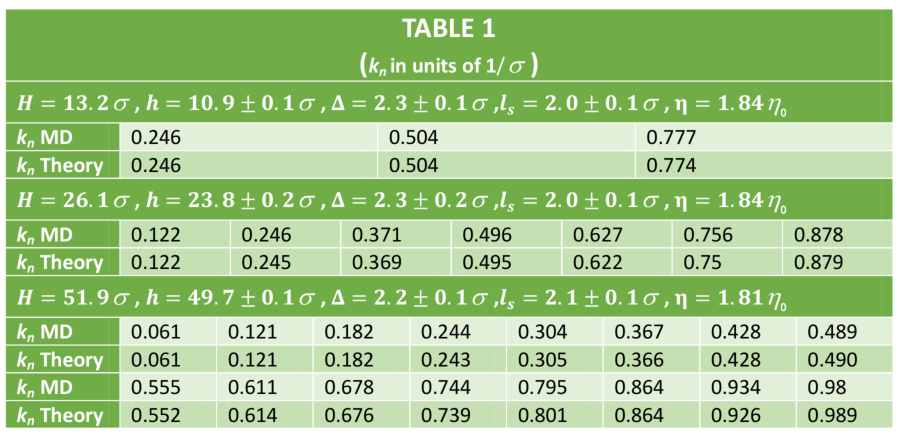
\includegraphics[width=1.0\textwidth]{fig/table-1.pdf}
  \end{figure}
  Theory: $
      \bluec{\tan (k_n h) = -k_n l_\slip}
    $
\end{frame}


\begin{frame}{模拟结果} {厌水固壁}
  \begin{figure}
    \centering
    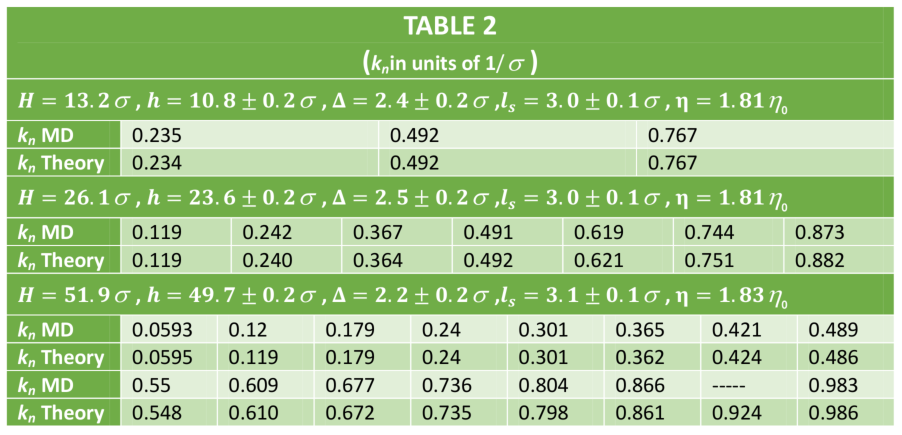
\includegraphics[width=1.0\textwidth]{fig/table-2.pdf}
  \end{figure}
  Theory: $
      \bluec{\tan (k_n h) = -k_n l_\slip}
    $
  \end{frame}


\begin{frame}
  \centerline{\bluec{\Huge 谢谢!}}
\end{frame}

}
\end{document}